\documentclass[11pt]{article}
\usepackage{eacl2017}
%\usepackage{natbib}
\usepackage{times}
\usepackage{url}
\usepackage{latexsym}
\usepackage{xspace}
\usepackage{multirow}
\usepackage{paralist}
\usepackage{amsmath}
\usepackage{graphicx}
\usepackage{url}
\usepackage[toc,page]{appendix}

\eaclfinalcopy % Uncomment this line for the final submission
%Position of pdflatex: /Library/TeX/Root/bin/x86_64-darwin

\newcommand\BibTeX{B{\sc ib}\TeX}


\newcommand\original{\textsc{Original}\xspace}
\newcommand\twitter{\textsc{Twitter}\xspace}

\newcommand\glove{GloVe\xspace}

\newcommand{\eqnref}[1]{Equation~\ref{#1}}
\newcommand{\figref}[1]{Figure~\ref{#1}}
\newcommand{\figsref}[2]{Figures~\ref{#1} and \ref{#2}}
\newcommand{\posciteauthor}[1]{\citeauthor{#1}'s}
\newcommand{\poscite}[1]{\citeauthor{#1}'s \citeyearpar{#1}}
\newcommand{\secref}[1]{Section~\ref{#1}}
\newcommand{\secsref}[2]{Sections~\ref{#1} and \ref{#2}}
\newcommand{\sentref}[1]{(\ref{#1})}
\newcommand{\tabref}[1]{Table~\ref{#1}}
\newcommand{\tabsref}[2]{Tables~\ref{#1} and \ref{#2}}


\title{Detecting unauthorized users on social media using textual data}

\author{Milton King  \\
Faculty of Computer Science, University of New Brunswick\\
Fredericton, NB E3B 5A3, Canada\\
\tt{milton.king@unb.ca}}

%To do
%Read a paper that uses OneClassSVM
%Different type of media or data that used author verification
%Cite sklearn: http://scikit-learn.org/stable/about.html#citing-scikit-learn

%\date{Nov. 27, 2017}

\begin{document}


\maketitle

\begin{abstract}
Although social media platforms can assist organizations' progress, it also makes them vulnerable to unauthorized users gaining access to their account and posting as the organization. This can have negative effects on the company including the defacing of a public appearance and a decrease in profit. An issue in this scenario is that once an attacker gains access to a social media account, they are able to post any content from that account. I propose an author verification in the realm of blog posts to detect and block unauthorized users based on the textual content of their unauthorized post. I compare four models -- two of which are novel to author verification. I show that a word embedding-based model can outperform two baselines, which include an all-in-one baseline and a model that performed well on an author verification shared task. I also describe how such an author verification system can be applied to a generic social media platform.

\end{abstract}

\section{Introduction}
There have been many cases of unauthorized personnel gaining access to social media accounts and posting content posing as the true owner of the account. An inappropriate post from a social media account can cause the defacing of a public image for both an individual and organization as well as the possibility for a loss of profit for the latter. In this work, I show that word embeddings can be applied to author verification, which involves determining the true author of a text, to better protect against unauthorized users posting from a social media account. More specifically, a model that is trained on known documents --documents belonging to the authorized author-- must predict if an unknown document --document whose identity is unknown at the time-- belongs to the authorized author. In this paper, I discuss the motivation for this work, a literature review surrounding this topic, information pertaining to the experiment that includes the research plan, design component, and implementations. I finish by concluding my findings as well as discussing the direction that this work can taken such as steps to possibly better my results and other methods that can be implemented to better protect social media accounts. I also provide a demonstration on how an author verification system can be used to protect a social media account.

\section{Motivation}

Many organizations now use social media to aid in their progression and success, while many individual users use social media as representing themselves on a social media platform. This however comes with the cost that any posts made by an account belonging to an organization or individual represents them regardless of who was the actual author of a post according to the public. Two instances where an unauthorized personnel gained access and posted from the social media account of an organization are the two tweets from McDonald's and Associated Press as see in in Figure \ref{mcDonalds} and \ref{press}. This can be harmful to the image of an individual or company and could potentially cost a reduction in profit, which is the case in the Associated Press incident. Shortly after this tweet from Associated Press was published, nearly 130 billion dollars with of stocks were temporarily lost \cite{financialTimes}. This one example shows the power that one individual has if they are granted access to a social media account that belongs to an organization such as Associated Press.  Although verification by passwords are implemented to protect social media accounts, these are not completely secure for few reasons. A user may not log out of their account when not using it and therefore anyone with possession of their device, such as a phone, has access to their social media account. Another reason could be that a social media account is hacked and therefore can be controlled by an unauthorized person. A defacing post could also be published from an authorized employee that wants to hurt the company that they work for. Most common social media accounts are protected by a single layer --the login process-- which grants the user full control of the publishing feature once they are past the login press. This is why I propose an author verification system that predicts if a post from a social media account is the legitimate author or an imposter after the account has been accessed by an unauthorized user. This system does not stop the social media account from being accessed by an unauthorized user but rather is a form of damage control to block unauthorized users from posting from social media accounts. This system will use author verification to predict if a text being published does belong to the authorized user, and if it predicts that it does not belong to the authorized user then a lockout occurs so that a secondary password is required to publish anything more from the account. 

%[Discuss number of social media accounts hacked] 

\begin{figure}
  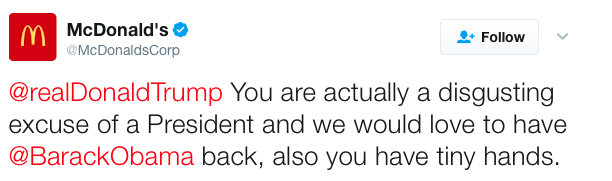
\includegraphics[width=\linewidth]{./mcDonalds}
  \caption{Tweet sent from an unauthorized user on the McDonald's Twitter account. Image taken from http://money.cnn.com/2017/03/16/ technology/mcdonalds-trump-tweet/}
  \label{mcDonalds}
\end{figure}

\begin{figure}
  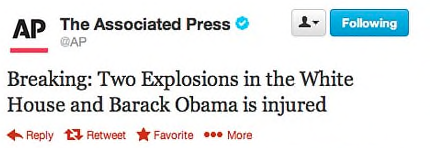
\includegraphics[width=\linewidth]{./associatedPress}
  \caption{Tweet sent from an unauthorized user on the Associated Press' Twitter account. Image taken from http://www.telegraph.co.uk/finance/markets/ 10013768/Bogus-AP-tweet-about-explosion-at-
the-White-House-wipes-billions-off-US-markets.html}
  \label{press}
\end{figure}

\section{Literature Review} \label{litReview}
A simple post can harm an organization \cite{oehri2012social}, whether it be from an authorized user or an unauthorized user. The insider threat in social media is when an authorized user of a social media account is responsible for harming an organization through the use of their social media account. This could be intended or accidental as in the case where an email was sent from Adidas with the title \textit{Congrats, you survived the Boston marathon!}. Some may see this as being perfectly acceptable in society, but others would associate it with the bombing that occurred at the Boston marathon in 2013. The insider threat exists in all realms of an organization where a person can harm a company from with the organization. \cite{gritzalis} evaluates personality traits of a social media user, specifically a Twitter user, to determine if they are or will become an insider threat to an organization by observing their behavior in social media. This work does not follow my work's direction but it is another method in protecting one's assets by analyzing social media. The insider threat is a serious issue for organizations, but this paper will focus on unauthorized users gaining access to a social media account.

\cite{Schmid:2015} used author attribution in the domain of emails, which they propose could be used by law enforcement as evidence against a subject. Their setup is slightly different than mine because, they are given documents from multiple authors as training data, while models in my experiment only see documents from the one authorized author for training. They use multiple associated rules, where each rule uses a feature for classification and a threshold to compare to. For example, if an author has 90\% of their emails containing 3 paragraphs then a rule can say that if a given email contains 3 paragraphs and the rule passes some threshold, then the email could belong to them. They performed rule pruning to remove rules that do not distinguish between authors well. Some of the features that were used include punctuation, n-grams, spelling errors, and rare word sequences. They used accuracy as their evaluation metric, which is one of the metrics that I use.

PAN\footnote{\url{http://pan.webis.de}} is an organization that releases tasks for researcher to work on and test their models. In 2013, PAN released an author verification task \footnote{\url{http://pan.webis.de/clef13/pan13-web/author-identification.html}}. In this task, models need to predict if a given document belongs to the author of a set of known documents \cite{Stamatatos_e.:overview}. In this shared task, their dataset consists of documents written in three different languages --English, Greek, and Spanish. A model is given a few documents --all written in the same language-- that belong to the same author for training and need to predict if a given document, which is also in the same language, belongs to the original author. The documents are either from textbooks, newspapers, or short fictions. They had 18 submissions for this task that vary in approaches. \cite{layton:2013} used a weighted local n-gram ensemble model. Local n-gram models represent an author by the most frequent n-grams --a set of \textit{n} number of characters or words-- and predicts if a document belongs to this author based on these n-grams. Their system contained multiple models, where each model is associated with a trained weight that is used to measure how trusting their prediction is. The predictions and weights are then used to determine the final prediction. Similarly, \cite{halvani:2013} used an ensemble of KNN classifiers, where each KNN model used a different feature such as prefixes, suffixes, part-of-speech, and character n-grams. \cite{maitra} also recruited machine learning techniques for their model, which was applied to the author verification task from PAN in 2015\footnote{\url{http://pan.webis.de/clef15/pan15-web/index.html}}. They used features such as punctuation count, punctuation ratio, long sentence to shot sentences ratio, and n-grams. These features are then used in a random forest classifier.

Pan also released an author verification task similar to the one in 2013 \footnote{\url{http://pan.webis.de/clef14/pan14-web/author-identification.html}}. This task again consisted of a multilingual dataset --containing text in English, and Spanish-- and was evaluated using F-score like the 2013 task \cite{pan2014}. Their dataset consists of documents from social media, blogs, Twitter, and hotel reviews. Following suit, my dataset for my experiment is blogs. They used the model from \cite{coling2014} as a baseline, which performed well on the 2013 task. This model uses a word occurrence dissimilarity that determines the dissimilarity between two documents based on the frequency of words. It uses this measurement to compare each known document against all other known documents and records the maximum dissimilarity. When given an unknown document, each document's dissimilarity is calculated with the unknown document and then divided by the known document's maximum dissimilarity to give a dissimilarity ratio. This dissimilarity ratio is calculated for all known documents and then averaged and compared to a dissimilarity threshold. If the ratio is less than the threshold, then the unknown document is labeled as belonging to the author, otherwise it is labeled as not belonging to the author. This model claims that if an unknown document is more similar to known documents then other known documents similarity score to known documents then the unknown document is labeled as belonging to the author. This model is used as a baseline in my experiment. \cite{castro} also used a similarity measurement for all documents of the known author but used feature vectors. The features used include prefixes, suffixes, and auxiliary words. They test a variety of similarity metrics such as Dice, Jaccard, Tani, cosine, Euclidean and minmax --with Jaccard usually achieving the best results. \cite{castillo:2014} approached this task using a variety of features to represent a document such as prefixes, suffixes, punctuation marks, and n-grams. A vector representation of these features are then used with a similarity metric to determine a similarity score. If this score is greater than some threshold then the document is classified as belonging to the author. This method was unsupervised, unlike \cite{moreau}, who used features such as n-grams and word length with a support vector machine as a classifier.    

The task of identifying which documents belong to a given author can also be seen as an outliers detection task, where a model must determine which documents are not related to a set of documents. \cite{Zhuang} segment a document into phrases that exhibit some semantic importance and then embed the the phrases using a neural network. The embeddings of documents are then compared using cosine similarity. Embeddings are vector representations of words, which are often generated by using artificial neural networks. The embeddings can be of words \cite{Mikolov+:2013b}, sentences \cite{Kiros+:2015}, paragraphs \cite{Le:Mikolov:2014}, or the context of words \cite{melamud2016context2vec}. Each of these models work with the idea that text that occurs near each other will have similar meaning. My proposed model uses word2vec's skip-gram embeddings from \cite{Mikolov+:2013b}, which uses a feed forward artificial neural network where the input is a word and the model predicts the surrounding words. Averaging word embeddings can be used as a vector representation of text as shown in \cite{jabri2016revisiting} and \cite{king-cook:2017}.



There are many different types of documents of which author verification can be applied. This could be emails \cite{Schmid:2015}, edited text such as newspapers or textbooks \cite{Stamatatos_e.:overview}, tweets \cite{gritzalis}, or blogs \cite{pan2014}. Each domain serves its purpose and can be used for author verification. I will be performing my experiments on blogs, but not the same dataset as \cite{pan2014} because the number of known documents for an author never exceeds ten in their dataset. This is an unrealistic environment, where it is common for an author on social media to have posted more times than ten. Blogs are an interesting domain to work in as they appear in many different sizes, are written from people from varying demographics, and can be either formal or informal. This is separate form emails as they usually appear with some degree of formality.



%Discuss embeddings

\section{Research Plan}
In this experiment, I will show that word embeddings can be used for author verification in social media, which in turn can be used to better protect social media accounts from impersonators. Four models will be applied to the dataset --two baselines and two novel approaches. These models will be compared using a variety of evaluation metrics --F-score, precision, recall, and accuracy-- to determine if word embeddings can benefit author verification in social media. Each model will be given documents of a single author to train on and then be given a set of documents to predict if each document belongs to the given author or not. The dataset that the experiments will use is generated from a blog corpus and is further explained in Section \ref{DATASET}. 

\section{Design Component}
In this section, I will first describe the dataset and how it was generated. I will then explain the experiment's setup as well as how each model is applied in the experiment.
%How to perform the experiments. The steps
\subsection{Dataset} \label{DATASET}

The dataset of my experiment consists of blogs from the corpus that was used in the work of \cite{schler2006effects}. This corpus is ideal for this task because it contains text from a form of social media, any authors, and many blog posts from an author. This allows many training documents for each author as well as many different authors to evaluate on. To generate the dataset, I first pull out all authors that have more than 300 posts that contain more than 100 words to ensure enough material to train on. This resulted in 103 authors. I then selected ten of these authors for the development set (Dev) and 93 authors in the test set (Test).

\subsection{General Setup}
Each model is applied to both the Dev set as well as the Test set. For each dataset, the model will have between 255 and 500 documents for each author to train on. The model only trains on one author at a time. The model is then given a set of randomly selected unknown documents, where half belong to the given author and half do not belong to the given author. Again, unknown documents are documents, whose author is unknown to the model. These unknown documents are not present in the training set. The model must classify each unknown document as belonging to the given author or not.  A single run of an author involves predicting one set of documents for one author. Accuracy, precision, recall, and F-score are calculated for a single run of an author. This run is then repeated five times and the evaluation metrics' results are averaged over the five runs. This process is repeated for each author in a dataset and the final average of the evaluation metrics over all authors are calculated and reported. 

\subsection{Applying Models}

The models are used in the experiments in different ways. The all-in-one model simply labels all given documents as belonging to author. The second baseline which will be called the Jankowska method from hereon, uses a dissimilarity comparison to classify unknown documents. The two novel models use word embeddings and an SVM for classifying unknown documents. I will now describe how each model is used in more detail.

\subsection{Jankowska Method}\label{Jankowska}
The second baseline used in this experiment is the Jankowska method, which was described in section \ref{litReview}, and uses a word occurrence dissimilarity which I'll call \textit{diff} that determines the dissimilarity between two documents based on the frequency of words as seen in figure \ref{diff}. The Jankowska model uses the \textit{diff} measurement to find the maximum dissimilarity for each known document. When given an unknown document, each document's dissimilarity is calculated with the unknown document using \textit{dff} and then divided by the known document's maximum dissimilarity to give a dissimilarity ratio. This dissimilarity ratio is calculated for all known documents and then averaged and compared to a dissimilarity threshold. If the ratio is less than the threshold, then the unknown document is labeled as belonging to the author, otherwise it is labeled as not belonging to the author. This threshold needs to be tuned.

\begin{figure}[h!]\label{diff}
  \caption{\textit{diff} calculation by Jankowska for two documents $D_1, D_2$. $x$ is a word and $fD(x)$ is the frequency of a word in a document.}
  ${diff(D_1, D_2)= \sum_{x\in(D_1 \cup D_2)}{(\dfrac{fD_1(x)-fD_2(x)}{\frac{fD_1(x)+fD_2(x)}{2}})}^2}$
\end{figure}

\subsection{Word Embedding Models}
I applied two different methods that involve word embeddings. The first model, which will be called the word2vec model, represents each document in the training set as an average of embeddings of words in the document --excluding stopwords. Stopwords are frequent words, such as \textit{the, a}, and \textit{is}, that can lead to biases towards documents appearing more similar due to the commonality of stopwords in the English language. The word embeddings are trained on a snapshot of Wikipedia. All of the vector representations of the training documents are used as input to scikit-learn's one-class-SVM \cite{scikit-learn}, which will be used as the model's classifier. Given an unknown document, the embeddings of the words in the document are averaged --again excluding stopwords-- and then used as input to the trained one-class-SVM, which then predicts if the document belongs to the author or not. One-class-SVM's only require seeing the instances of one class in a classification problem, therefore making it an ideal classifier for this problem. Similarly to the dissimilarity threshold, the kernel coefficient of the SVM must also be tuned. The final model, which will be called word2vec+tf-idf, is similar to the word2vec method that was explained, but also recruits the use of term frequency-inverse document frequency (tf-idf). Tf-idf is the number of times a word occurs in a document at test time divided by the number of documents that the word was seen in during training. Instead of averaging just the word embeddings to represent a document, it divides each word embedding, which is first normalized, by the word's associated inverse document frequency value. The term frequency is multiplied by the inverse document frequency through the addition of the word embedding each time the word is seen. Tf-idf is used to give more weights to less common words as they can be good indicators of the actual author. Tf-idf has proven to be a powerful baseline in semantic analysis. The idf values were trained on documents from the Dev set.

\subsection{Evaluation metrics}\label{metrics}
In the experiments, I used a variety of evaluation metrics --including precision, recall, F-score, and accuracy-- to better analyze the performance of each model. In these experiments I treated a true positive as being a document that was correctly labeled as belonging to the given author. Therefore, the precision is equal to the number of correctly labeled documents belonging to the author divided by the sum of the correctly labeled documents belonging to the author and the number of incorrectly labeled documents that do not actually belong to the author. Formally, the precision is $\frac{tp}{tp+fp}$ , where $tp$ is the true positive and $fp$ is the false positive. Similarly, the recall is measured as  $\frac{tp}{tp+fn}$, where $fn$ is the false negative. Recall is sensitive to incorrectly labeling documents that belong to the author as not belonging to the author while the precision metric is sensitive to incorrectly labeling documents the don't belong to the author as belonging to the author. The F-score is the harmonic mean of the precision and recall, which is calculated as $2\frac{precision*recall}{precision+recall}$ giving a range from the least score 0 to a maximum score of 1. I used accuracy as the fourth measure, which is calculated by $\frac{tp+fp}{number of documents}$ and captures how well a model can classify a document regardless of the class. This metric can be a poor performance analyzer if the dataset is not biased towards a class. For example, if there were 9 positive classes and 1 negative class, then a model that classified every instance as being positive would have a high accuracy but does not perform well in capturing information pertaining to the negative class. Both the Dev and Test dataset contain an equal distribution between the positive and negative classes --half positive and half negative-- and therefore  allowing accuracy to be a useful metric for these datasets.

\section{Implementation}
In this section, I will discuss parameter tuning for all models as well as the experimental results on both the Dev and Test datasets. 
\subsection{tuning}
The first experiments performed involved the tuning of Jankowska's dissimilarity threshold and the one-class-SVM's kernel coefficient. The F-score for the tuning of the Jankowska method and the embedding-based methods on the Dev set are shown in Figure \ref{magtuning}, \ref{SVMtuning}, and \ref{tfidftuning} respectively. The magdelena method achieves its highest F-score of $0.6663$ using a dissimilarity threshold of $1$, while both the word2vec and word2vec+tfidf methods achieve their highest F-score of $0.5395$ and $0.5954$, respectively, using a kernel coefficient of $0.001$. These tuned parameters will be used for all experiments discussed from hereon.

\begin{table}
\begin{center}
\small
\setlength{\tabcolsep}{2pt}
\begin{tabular}{c|c}
Threshold & F-score\\ 
\hline
0.1 & 0.0493\\
0.2 & 0.3486\\
0.4 & 0.6127\\
0.6 & 0.6592\\
0.8 & 0.6655\\
1.0 & \textbf{0.6663}\\
1.2 & 0.6660\\

\end{tabular}
\caption{F-score using the Jankowska method with different values for the dissimilarity threshold with the highest F-score in bold. \label{magtuning}}
\end{center}
\end{table}

\begin{table}
\begin{center}
\small
\setlength{\tabcolsep}{2pt}
\begin{tabular}{c|c}
Kernel Coefficient & F-score\\ 
\hline
0.0001 & 0.5080\\
0.001 & 0.5395\\
0.01 & 0.5387\\
0.1 & 0.5376\\
1 & 0.5375\\
10 & 0.5383\\


\end{tabular}
\caption{F-score using the word2vec method with different values for the kernel coefficient of the one-class-SVM with the highest F-score in bold. \label{SVMtuning}}
\end{center}
\end{table}

\begin{table}
\begin{center}
\small
\setlength{\tabcolsep}{2pt}
\begin{tabular}{c|c}
Kernel Coefficient & F-score\\ 
\hline
0.0001 & 0.4906\\
0.001 & \textbf{0.5954}\\
0.01 & 0.5553\\
0.1 & 0.4792\\
1 & 0.5106\\
10 & 0.5144\\


\end{tabular}
\caption{F-score using the word2vec+tf-idf method with different values for the kernel coefficient of the one-class-SVM with the highest F-score in bold. \label{tfidftuning}}
\end{center}
\end{table}

\subsection{Experimental Results}

I will now discuss the performance of the models on both datasets using all the evaluation metrics discussed in section \ref{metrics}. Looking at the results on the Dev set in Figure \ref{devResults}, the word2vec method outperforms all models in terms of accuracy with $54.3\%$ but performs worse when incorporating tf-idf. The baselines, all-in-one and Jankowska, perform similar to each other with an accuracy of $50\%$. This makes sense, since they both predict all or most documents as belonging to the author. In terms of F-score, the all-in-one baseline achieves the best performance with $0.667$ with Jankowska performing similarly with $0.666$. Both of the word2vec-based models perform worse here, but word2vec improves when tf-idf is used. The word2vec model shows that it is better at predicting which documents do not belong to the author by achieving the highest precision of $0.580$ but the lowest recall of $0.525$. Incorporating the use of tf-idf significantly raises the recall to $0.801$, but still falls short of the perfect recall of the all-in-one baseline. 

\begin{table}
\begin{center}
\small
\setlength{\tabcolsep}{2pt}
\begin{tabular}{c|cccc}

&All-in-one & Jankowska & Word2vec & Word2vec+tfidf\\
\hline
Accuracy & 0.500 & 0.500 & \textbf{0.543} & 0.528 \\
F-score & \textbf{0.667} & 0.666 & 0.540 & 0.595 \\
Precision & 0.500 & 0.500 & \textbf{0.580} & 0.535 \\
Recall &  \textbf{1.000} & 0.998 & 0.525 & 0.801\\
\hline


\end{tabular}
\caption{Evaluation on the Dev set. \label{devResults}}
\end{center}
\end{table}

Looking at the results on the Test set in Figure \ref{testResults}, they tell a similarly story as the results for the Dev set. Again Word2vec achieves the highest accuracy and precision, where the former is decreased when adding the assistance of tf-idf and the latter is increased significantly with the assistance of tf-idf. Jankowska achieves the highest F-score over the all-in-one baseline, which is accredited to Jankowska's increase in precision over the all-in-one baseline.

\begin{table}
\begin{center}
\small
\setlength{\tabcolsep}{2pt}
\begin{tabular}{c|cccc}

&All-in-one & Jankowska & Word2vec & Word2vec+tfidf\\
\hline
Accuracy & 0.500 & 0.504 & \textbf{0.562} & 0.512 \\
F-score & 0.667 & \textbf{0.668} & 0.531 & 0.625 \\
Precision & 0.500 & 0.502 & \textbf{0.600} & 0.515 \\
Recall & \textbf{1.000} & 0.997 & 0.489 & 0.861\\
\hline


\end{tabular}
\caption{Evaluation on the Test set. \label{testResults}}
\end{center}
\end{table}

As a further analysis of these models, I evaluated their performance using the same metrics but switching what is considered as a true positive. The results in Figure \ref{unauthorized} treats the true positive case as correctly identifying which documents do not belong to the author. It is important to keep in mind that these models are still tuned to perform well in terms of the original F-score used in Figures \ref{magtuning}, \ref{SVMtuning}, and \ref{tfidftuning}. The results on the Test set in Figure \ref{unauthorized} show that both the all-in-one and Jankowska methods perform poorly with all metrics. The word2vec model achieves the highest F-score of $0.582$ and recall of $0.635$, which are both lowered with adding the use of tf-idf. However,  the addition of tf-idf does assist word2vec in terms of the precision. 

\begin{table}
\begin{center}
\small
\setlength{\tabcolsep}{2pt}
\begin{tabular}{c|cccc}

&All-in-one & Jankowska & Word2vec & Word2vec+tfidf\\
\hline
F-score & 0.000 & 0.022 & \textbf{0.582} & 0.207 \\
Precision & 0.000 & 0.350 & 0.544 & \textbf{0.581} \\
Recall & 0.000 & 0.012 & \textbf{0.635} & 0.163\\
\hline


\end{tabular}
\caption{Unauthorized setup on Test set. \label{unauthorized}}
\end{center}
\end{table}

To compare the models' F-score for both setups, I averaged both F-scores for an overall F-score measure. This and the accuracy can be used to give a more general analyses of the models' performance. Shown in Figure \ref{average}, word2vec achieves the highest average F-score of $0.556$. Adding tf-idf to word2vec hurts the average F-score bringing down to $0.416$. The Jankowska method outperforms the all-in-one baseline with a score of $0.345$ compared to the all-in-one's score of $0.333$.


\begin{table}
\begin{center}
\small
\setlength{\tabcolsep}{2pt}
\begin{tabular}{c|c}

Model & Average F-score\\
\hline
All-in-one &  0.333\\
Jankowska & 0.345\\
Word2vec &  \textbf{0.556}\\
Word2vec+tfidf & 0.416\\
\hline


\end{tabular}
\caption{Average F-score on Test set. \label{average}}
\end{center}
\end{table}

\section{Demonstration}
A simulation of how an author verification can be applied to a social media application is seen in Figures \ref{demo1}, \ref{demo2}, \ref{demo3}, \ref{demo4}, and \ref{demo5}. In Figure \ref{demo1}, the documents that belong to the authorized user are loaded into the system and the application waits for a post to be entered. In Figure \ref{demo2}, a post is entered that does belong to the authorized author and was not included in the documents that the model was trained on. In Figure \ref{demo3}, the application verifies that the post was published. Figure \ref{demo4} shows a post being entered that does no belong to the authorized user. In Figure \ref{demo5}, the application predicts that the post was not written by the authorized user and therefore locks the social media account until the user can verify that they are the authorized user with a username and password. An added security measure would insist that this password is different then the original password that is used to regularly sign into the account. The code for this application, which involves the code on how it performs author verification using the word2vec method, is given in Figures \ref{demoCode1} and \ref{demoCode2}.

\section{Conclusions\label{sec:conclusions}}
Unauthorized use of social media accounts can have serious effects such as defacing an image or loss of profit such as the McDonald's and Associated Press incidences. The current one step authorization is clearly not enough protection for one's social media account. Author verification can be used as a secondary protection to limit the effect that unauthorized users make while they have access to a victim's account by locking out unauthorized users if a piece of text is sent that is predicted to not belong to the true author. I applied four different models to an author verification to show that these models can be used to better secure a social media account belonging to a single user. The word2vec model achieved the highest score in terms of both average F-score and accuracy. This shows that it is better at classifying both classes and not only one class like the all-in-one and Jankowska baselines. The use of tf-idf has been known to work well on many natural language processing tasks, but unfortunately it does not provide much assistance in these experiments. This could be due to the small amount of training data that they were trained on. The Jankowska method showed that it was too sensitive to sets of documents for training that contain at least one document that was rated as highly dissimilar making all unknown documents appear more relatively similar. This sensitivity caused the model to predict most documents as belonging to the author. This could be due to a repost or a quote from another author, which would introduce words that would not be normally used by the true author. The benefit that all these systems have is their speed to classify a document. All models can classify a document with negligible delay in time, which is important for an application. A delay in time when using any software that implements an author verification model would drive users away from this system and therefore would not be easily adopted in the realm of social media. 

\section{Future work}
Protecting social media accounts by analyzing textual data does not stop at author verification. Similar methods could be applied to assist in analyzing text being sent from a social media account to detect the presence of sensitive topics or negative material. The issue regarding posts about sensitive issues can easily be displayed in the earlier described case involving Adidas involving the email with the title of \textit{Congrats, you survived the Boston marathon!}. A simple preliminary model could use the word occurrence of \textit{survive} and \textit{Boston marathon} to check if they have been used in any social media corpus as being labeled as sensitive. The latter task of detecting negative material, which is also known as sentiment analyses, can be used to detect if a social media account wants to send a document that contains negative sentiment. This could also be used in the case of the McDonald's incident, where negative terms were used against the current president of the United States.
There are a few modifications that could be made to better my models in the author verification task. This includes use of metadata, different training data for word embeddings, and different embedding model. The dataset is accompanied with metadata of each author as well as the time that each blog was posted. The former would be difficult to use with the current setup where a model only sees the one user during training, although if the model had access to more authors, a model could use the metadata about the authors to augment the vector representation of a document similarly to \cite{lynn}. The word embeddings used were trained on a snapshot of Wikipedia, but a more suitable corpus to train them on would be a corpus of blogs. A further experiment that would be interesting is to see how each model performs with different amounts of training data. This would show which models are preferred when access to training documents is limited. A social media detection system could therefore use one method when the author has posted a number of documents below a certain threshold and another method when they reach the threshold.


\section*{Acknowledgments}
I would like to thank Paul Cook for assisting me in this experiment.
%\begin{appendices}
%\section{Demonstration}



%\end{appendices}

\bibliography{./big}
\bibliographystyle{eacl2017}

\begin{figure}[h]
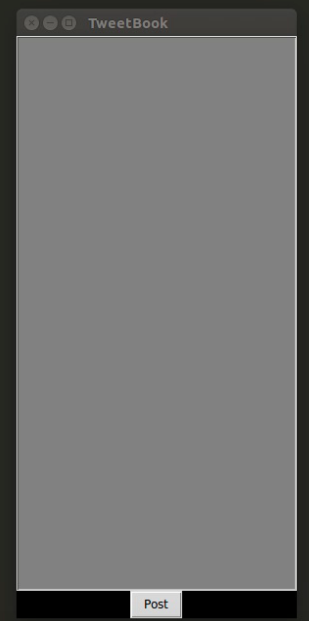
\includegraphics[width=50mm]{./Images/demo1}
  \caption{Simulation of a social media application for posting text.}
  \label{demo1}
\end{figure}

\begin{figure}[h]
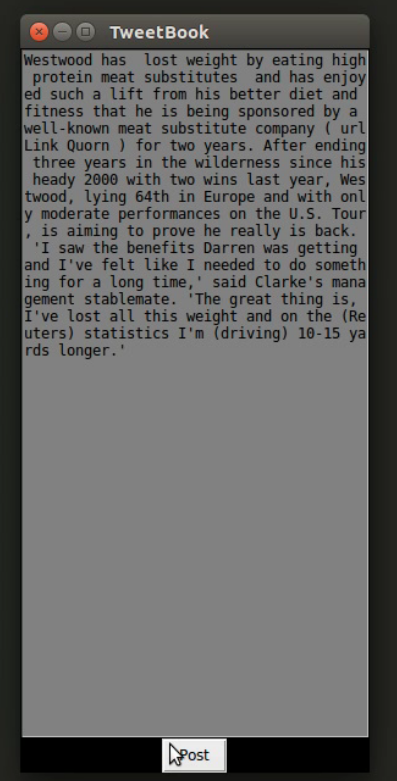
\includegraphics[width=50mm]{./Images/demo2}
  \caption{Attempting to send a post that belongs to the authorized user.}
  \label{demo2}
\end{figure}

\begin{figure}[h]
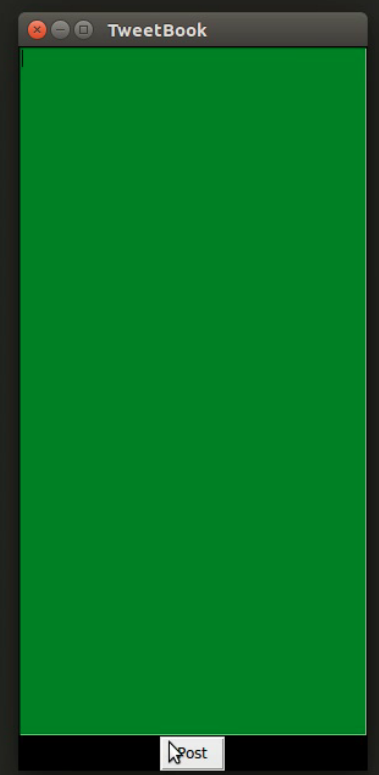
\includegraphics[width=50mm]{./Images/demo3}
  \caption{The post belonging to the authorized user was sent successfully.}
  \label{demo3}
\end{figure}

\begin{figure}[h]
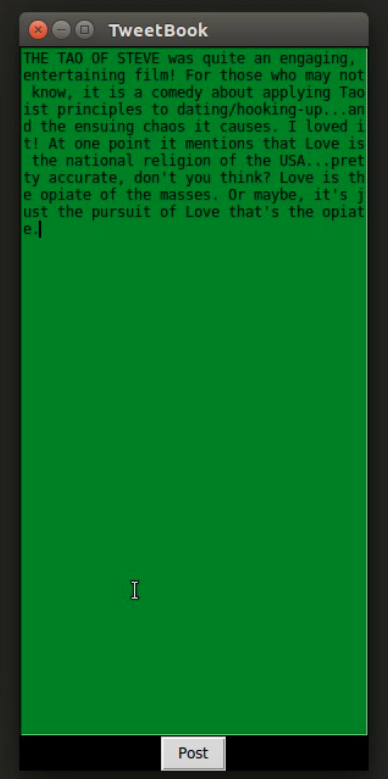
\includegraphics[width=50mm]{./Images/demo4}
  \caption{Attempting to send a post that does not belong to the authorized user.}
  \label{demo4}
\end{figure}

\begin{figure}[h]
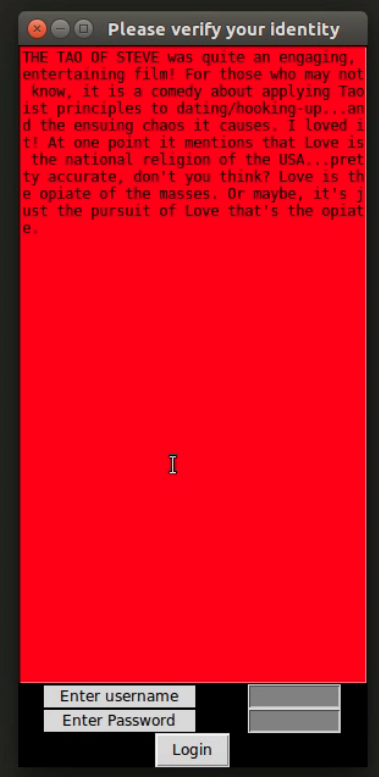
\includegraphics[width=50mm]{./Images/demo5}
  \caption{The post that does not belong to the authorized user failed to send and the user was locked out of the social media application until they can verify that they are the authorized user.}
  \label{demo5}
\end{figure}



%\section{Code for demonstration}
\begin{figure}
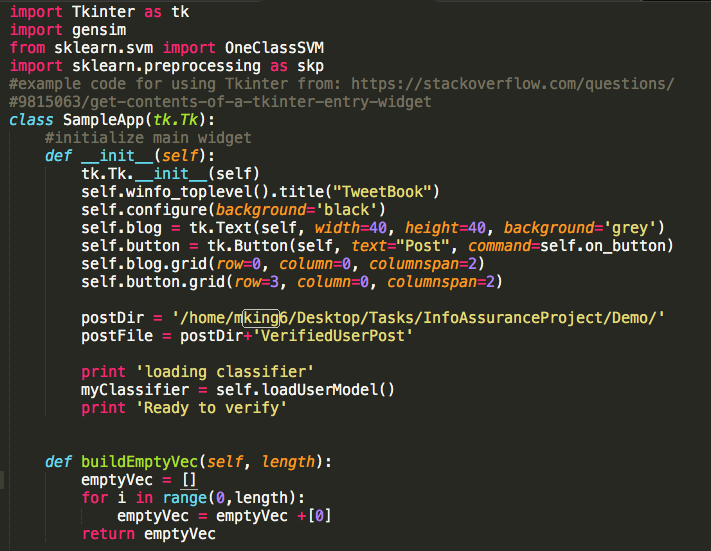
\includegraphics[width=\linewidth]{./Images/demoCode1}
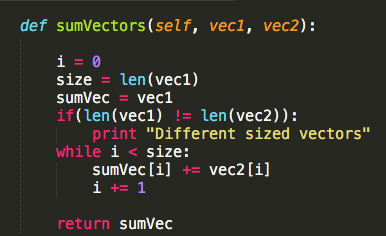
\includegraphics[width=\linewidth]{./Images/demoCode2}
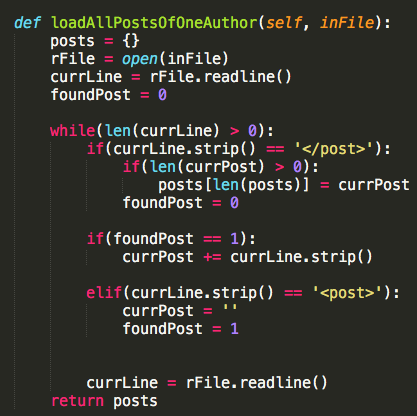
\includegraphics[width=\linewidth]{./Images/demoCode3}
  \caption{First half of the python code for the demonstration.}
  \label{demoCode1}
\end{figure}

\begin{figure}

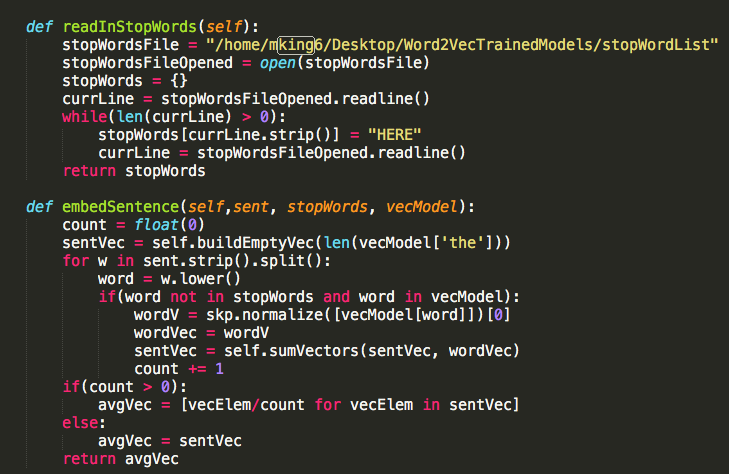
\includegraphics[width=\linewidth]{./Images/demoCode4}
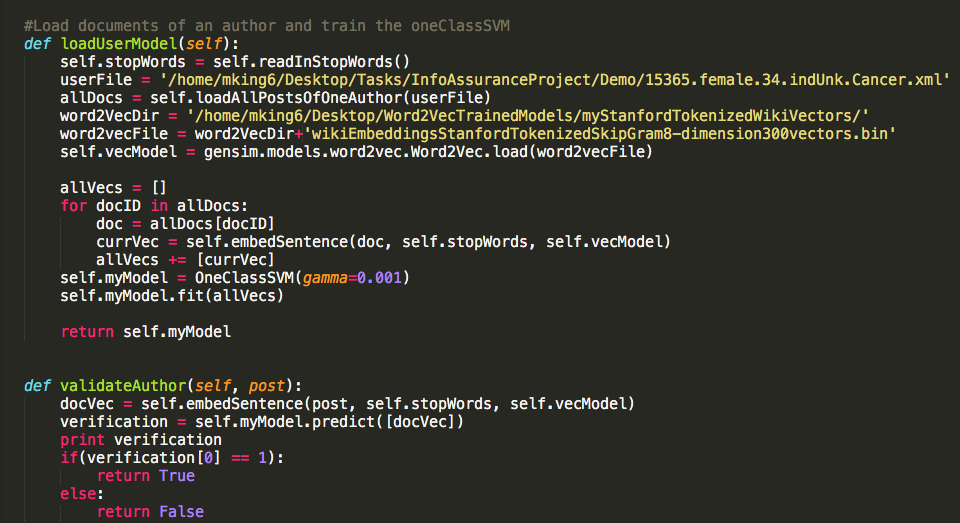
\includegraphics[width=\linewidth]{./Images/demoCode5}
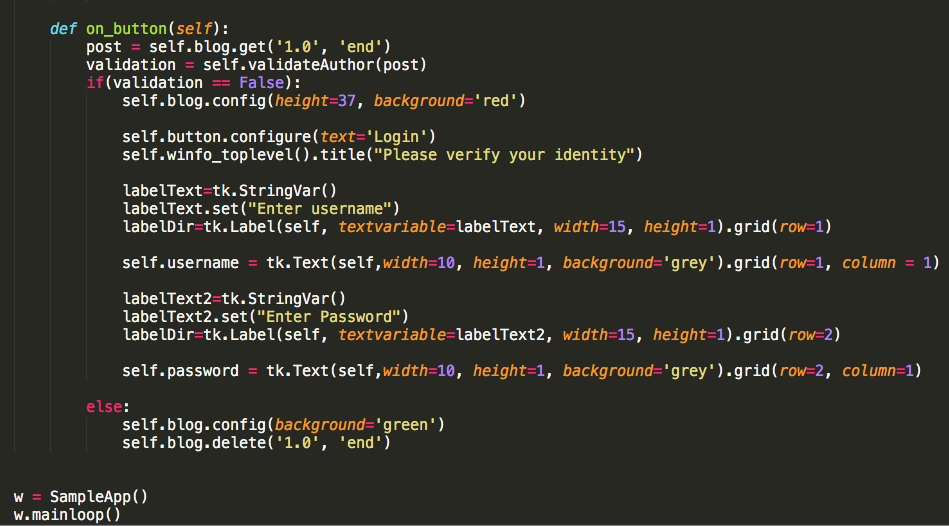
\includegraphics[width=\linewidth]{./Images/demoCode6}
  \caption{Second half of the python code for the demonstration}
  \label{demoCode2}
\end{figure}


\end{document}



